\resizebox{\linewidth}{!}{%
\begin{tikzpicture}[
  panelbox/.style={draw=black!45, line width=1.0pt, rounded corners=1.5pt, minimum width=3.9cm, minimum height=3.9cm},
  headertext/.style={font=\bfseries\small, align=center},
  chapterlabel/.style={font=\bfseries\footnotesize, black!55, align=center},
  desctext/.style={font=\footnotesize, align=center, text width=3.8cm},
  scaletext/.style={font=\bfseries\small},
]

% ============ panel frames (empty boxes to anchor content on) ============
\node[panelbox] (p1) {};
\node[panelbox, right=1.0cm of p1] (p2) {};
\node[panelbox, right=1.0cm of p2] (p3) {};
\node[panelbox, right=1.55cm of p3] (p4) {};

% ============ panel 1: AME -- fixed grid + attention entropy ============
% Same idea as the AdaGlimpse panel: a small underlying "scene" gives the
% masking/glimpse concept something concrete to reveal, rather than an
% entirely abstract grid. Only the two already-observed cells show a
% fragment of it, faithful to how a masked autoencoder actually works --
% everything else (including the entropy-selected cell) stays unseen.
\begin{scope}[shift={(p1.center)}]
  \def\g{0.62} % grid cell size
  \def\amescene{
    \fill[black!14] (-0.9,-1.24) -- (-0.2,-0.35) -- (0.5,-1.24) -- cycle;
    \fill[darkorange25512714, opacity=0.4] (-0.93,0.31) circle (0.22);
  }

  % mask everything first ...
  \foreach \i in {0,1,2,3} {
    \foreach \j in {0,1,2,3} {
      \fill[white] ({(\i-2)*\g},{(\j-2)*\g}) rectangle ++(\g,\g);
    }
  }
  % ... then reveal the scene only within the two observed glimpse cells
  \begin{scope}
    \clip ({(0-2)*\g},{(2-2)*\g}) rectangle ++(\g,\g);
    \amescene
  \end{scope}
  \begin{scope}
    \clip ({(1-2)*\g},{(1-2)*\g}) rectangle ++(\g,\g);
    \amescene
  \end{scope}

  \foreach \i in {0,1,2,3} {
    \foreach \j in {0,1,2,3} {
      \draw[black!35, line width=0.35pt] ({(\i-2)*\g},{(\j-2)*\g}) rectangle ++(\g,\g);
    }
  }
  % observed cells get a slightly heavier border so they read as "revealed"
  \draw[black!45, line width=0.6pt] ({(0-2)*\g},{(2-2)*\g}) rectangle ++(\g,\g);
  \draw[black!45, line width=0.6pt] ({(1-2)*\g},{(1-2)*\g}) rectangle ++(\g,\g);

  % step order badges make the *sequence* of glimpses explicit -- this is a
  % selection process, not a static pair of revealed cells
  \node[circle, fill=black!65, text=white, font=\tiny\bfseries, inner sep=1pt] at (-0.57,-0.06) {1};
  \node[circle, fill=black!65, text=white, font=\tiny\bfseries, inner sep=1pt] at (-1.18,0.57) {2};

  % entropy-selected next glimpse -- still unseen, just highlighted
  \fill[crimson2143940, opacity=0.55] ({(2-2)*\g},{(2-2)*\g}) rectangle ++(\g,\g);
  \draw[crimson2143940, thick] ({(2-2)*\g},{(2-2)*\g}) rectangle ++(\g,\g);

  % the model's current (entropy) belief drives the *next* glimpse choice --
  % an explicit arrow from the latest observation to the selected cell
  \draw[-{Latex[length=1.5mm]}, very thick, orange] (-0.7,0.44) to[bend left=14] (0.16,0.44);
\end{scope}

% ============ panel 2: Beyond Grids -- elastic, variable-size patches ============
\begin{scope}[shift={(p2.center)}]
  \draw[black!25, line width=0.35pt, fill=black!4] (-1.5,-1.5) rectangle (1.5,1.5);
  \draw[mediumpurple148103189, thick, fill=mediumpurple148103189, fill opacity=0.28] (-1.25,0.55) rectangle ++(0.95,0.85);
  \draw[steelblue31119180, thick, fill=steelblue31119180, fill opacity=0.28] (0.05,0.75) rectangle ++(0.5,0.5);
  \draw[forestgreen4416044, thick, fill=forestgreen4416044, fill opacity=0.28] (-0.35,-0.55) rectangle ++(1.35,0.85);
  \draw[darkorange25512714, thick, fill=darkorange25512714, fill opacity=0.28] (0.75,-1.3) rectangle ++(0.35,0.35);
  \draw[crimson2143940, thick, fill=crimson2143940, fill opacity=0.28] (-1.35,-1.35) rectangle ++(0.65,0.5);
\end{scope}

% ============ panel 3: AdaGlimpse -- coarse-to-fine continuous zoom ============
% A small abstract "scene" to zoom into (echoing the paper's real teaser: a
% sequence of glimpses converging on a subject), plus a genuine three-step
% coarse -> medium -> fine progression rather than a single before/after jump.
\begin{scope}[shift={(p3.center)}]
  \draw[black!25, line width=0.35pt, fill=black!4] (-1.5,-1.15) rectangle (1.5,1.15);
  % a couple of muted background shapes -- something concrete for the
  % glimpses to converge on, without competing visually with them
  \fill[black!14] (-1.15,-1.15) -- (-0.5,-0.1) -- (0.1,-1.15) -- cycle;
  \fill[black!11] (-0.05,-1.15) -- (0.5,-0.25) -- (1.05,-1.15) -- cycle;
  \fill[darkorange25512714, opacity=0.35] (0.82,0.72) circle (0.24);

  % coarse: the whole scene
  \draw[steelblue31119180, thick] (-1.5,-1.15) rectangle (1.5,1.15);
  \node[font=\tiny, steelblue31119180] at (-1.14,0.92) {coarse};

  % medium: narrows toward the subject
  \draw[mediumpurple148103189, thick] (-0.05,-0.25) rectangle (1.35,1.05);

  % fine: zoomed in on the subject itself
  \draw[crimson2143940, thick] (0.5,0.4) rectangle (1.18,1.0);
  \node[font=\tiny, crimson2143940] at (0.84,1.12) {fine};

  \draw[-{Latex[length=1.5mm]}, very thick, orange] (-0.85,-0.85) to[bend right=15] (-0.02,0.15);
  \draw[-{Latex[length=1.5mm]}, very thick, orange] (0.28,0.28) to[bend right=15] (0.68,0.55);

  % step order badges -- same language as the AME panel, making explicit
  % that this is a sequence of decisions, not a single before/after jump
  \node[circle, fill=black!65, text=white, font=\tiny\bfseries, inner sep=1pt] at (-1.4,-1.05) {1};
  \node[circle, fill=black!65, text=white, font=\tiny\bfseries, inner sep=1pt] at (0.02,-0.13) {2};
  \node[circle, fill=black!65, text=white, font=\tiny\bfseries, inner sep=1pt] at (1.11,0.46) {3};

  \node[draw=black!55, rounded corners=1pt, fill=black!4, font=\tiny, inner sep=2pt] at (0,-1.55) {RL (SAC)};
\end{scope}

% ============ panel 4: FlySearch -- UAV flying over open 3D world ============
% scale by height and clip to the panel square so it fills it fully, matching
% the other three (line-art) panels instead of sitting letterboxed inside.
\begin{scope}
  \clip ($(p4.center)+(-1.95,-1.95)$) rectangle ++(3.9,3.9);
  \node[inner sep=0pt] at (p4.center) {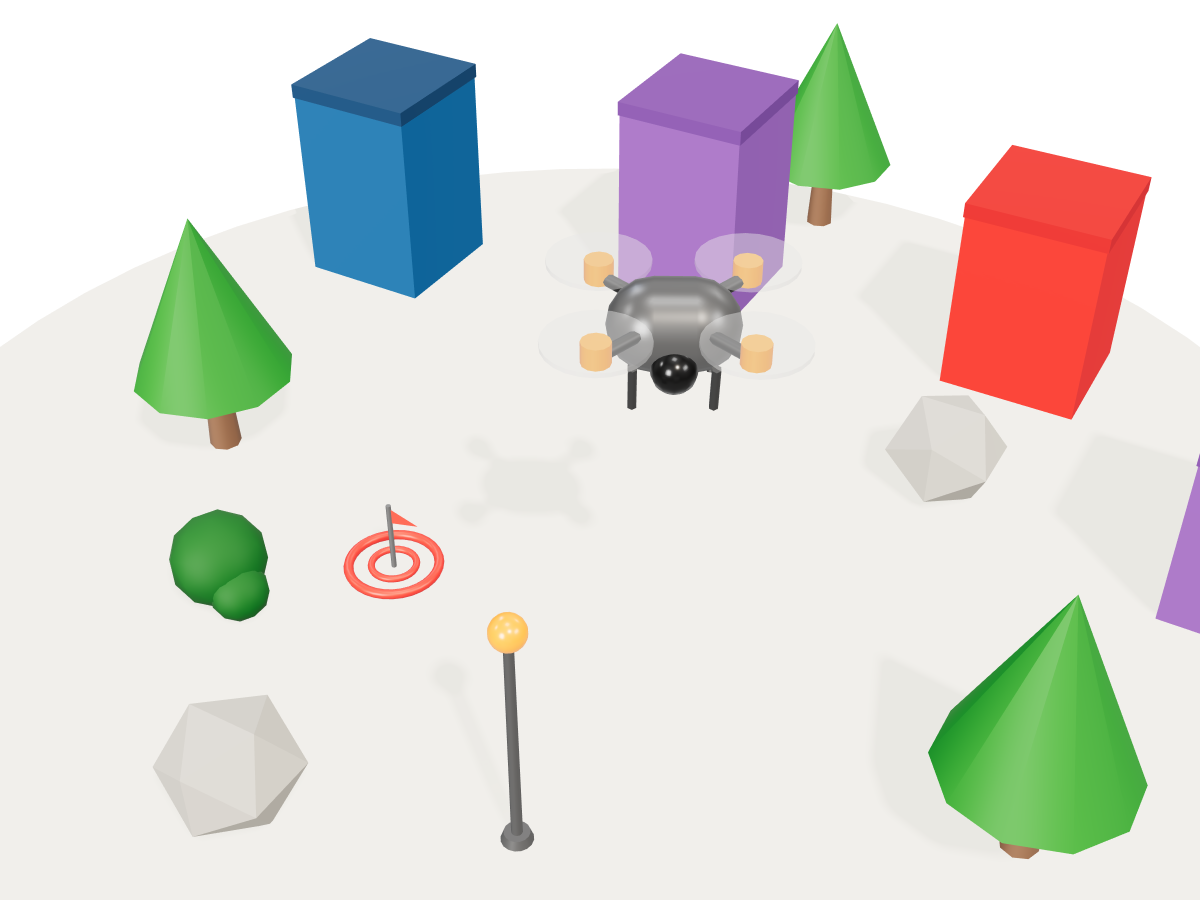
\includegraphics[height=3.9cm]{img/main/three/renders/flysearch_uav.png}};

  % search path overlay -- same numbered-arrow language as the other three
  % panels: 1 = starting position (the UAV), 2 = a waypoint en route,
  % 3 = the target it is searching for
  \draw[-{Latex[length=1.5mm]}, very thick, orange] ($(p4.center)+(0.18,0.78)$) to[bend right=8] ($(p4.center)+(-0.35,0.15)$);
  \draw[-{Latex[length=1.5mm]}, very thick, orange] ($(p4.center)+(-0.42,0.05)$) to[bend right=8] ($(p4.center)+(-0.75,-0.42)$);

  \node[circle, fill=black!65, text=white, font=\tiny\bfseries, inner sep=1pt] at ($(p4.center)+(0.26,0.82)$) {1};
  \node[circle, fill=black!65, text=white, font=\tiny\bfseries, inner sep=1pt] at ($(p4.center)+(-0.35,0.15)$) {2};
  \node[circle, fill=black!65, text=white, font=\tiny\bfseries, inner sep=1pt] at ($(p4.center)+(-0.6,-0.44)$) {3};
\end{scope}

% ============ headers ============
\node[headertext, above=0.28cm of p1] (h1) {AME (IJCAI 2023)};
\node[headertext, above=0.28cm of p2] (h2) {Beyond Grids (WACV 2025)};
\node[headertext, above=0.28cm of p3] (h3) {AdaGlimpse (ECCV 2024)};
\node[headertext, above=0.28cm of p4] (h4) {FlySearch (NeurIPS 2025)};

% chapter numbers above the titles -- Beyond Grids and AdaGlimpse are both
% Chapter 3, so they share a single, centred label rather than repeating it.
\node[fit=(h2)(h3), inner sep=0pt] (h23) {};
\node[chapterlabel, above=0.1cm of h1] {Chapter 2};
\node[chapterlabel, above=0.1cm of h23] {Chapter 3};
\node[chapterlabel, above=0.1cm of h4] {Chapter 4};

% ============ one-line descriptions ============
\node[desctext, below=0.3cm of p1] {fixed grid, exploration based on uncertainty reduction};
\node[desctext, below=0.3cm of p2] {variable-size patch encoder, free scale and position};
\node[desctext, below=0.3cm of p3] {adaptive coarse-to-fine exploration};
\node[desctext, below=0.3cm of p4] {open 3D world, vision-language object navigation};

% ============ bottom scale band ============
\node[fit=(p1)(p2)(p3), inner sep=0pt] (localfit) {};
\coordinate (bandy) at ($(p1.south)+(0,-2.25)$);
\draw[black!85, thick] (localfit.west |- bandy) -- (localfit.east |- bandy);
\node[scaletext, black!85, fill=white, inner sep=2pt] at ($(localfit.center |- bandy)$) {LOCAL SCALE};

\draw[black!85, thick] (p4.west |- bandy) -- (p4.east |- bandy);
\node[scaletext, black!85, fill=white, inner sep=2pt] at ($(p4.center |- bandy)$) {GLOBAL SCALE};

% light divider between panels 1 and 2 (Chapter 2 vs Chapter 3), much fainter
% than the local-to-global divider since it's a much smaller distinction.
\node[fill=black!22, inner sep=0pt, minimum width=0.6pt, minimum height=7.1cm, anchor=north,
      right=0.5cm of p1.east, yshift=0.1cm] {};

% heavier divider marking the local-to-global jump, between panels 3 and 4
\node[fill=black!70, inner sep=0pt, minimum width=1.1pt, minimum height=7.1cm, anchor=north,
      right=0.775cm of p3.east, yshift=0.1cm] {};

\end{tikzpicture}%
}
